\documentclass[11pt,a4paper]{article}

% ---------------------------------------------------------------------------
% Objective 5 report: on-device kiosk app and per-stage measurement
% Compile with:  pdflatex objective5_report.tex  (run twice for references)
% Figures are expected in ./figs/ (make_figs.py; screenshots from shots.py).
% ---------------------------------------------------------------------------

\usepackage[margin=2.4cm]{geometry}
\usepackage[T1]{fontenc}
\usepackage{mathpazo}
\usepackage{microtype}
\usepackage{graphicx}
\usepackage{booktabs}
\usepackage{tabularx}
\usepackage{xltabular}
\usepackage{array}
\usepackage{multirow}
\usepackage{xcolor}
\usepackage{enumitem}
\usepackage{amsmath,amssymb}
\usepackage{caption}
\usepackage{float}
\usepackage{tikz}
\usetikzlibrary{arrows.meta,positioning,shapes.geometric,fit,calc}
\usepackage{url}
\usepackage[hidelinks]{hyperref}

\definecolor{ink}{HTML}{0B0B0B}
\definecolor{ink2}{HTML}{52514E}
\definecolor{qblue}{HTML}{2A78D6}
\definecolor{qorange}{HTML}{EB6834}
\definecolor{qaqua}{HTML}{1BAF7A}
\definecolor{qred}{HTML}{C9302C}
\definecolor{boxfill}{HTML}{F3F7FD}
\definecolor{fixfill}{HTML}{EEF7EE}
\definecolor{warnfill}{HTML}{FDF0EA}

\captionsetup{font=small,labelfont=bf}
\setlist{itemsep=2pt,topsep=4pt}
\renewcommand{\arraystretch}{1.18}
\newcolumntype{L}{>{\raggedright\arraybackslash}X}
\newcommand{\met}{\textcolor{qaqua}{\textbf{met}}}
\newcommand{\missed}{\textcolor{qred}{\textbf{missed}}}
\newcommand{\na}{\textcolor{ink2}{n/a}}
\newcommand{\brand}{$\diamond\,\diamond\,\diamond$}

% Placeholder: replace before submission
\newcommand{\placeholder}[1]{\textcolor{red}{[#1]}}
\newcommand{\reportdate}{7 November 2026}

\title{\textbf{From an Evaluated Pipeline to an Offline Kiosk App}\\[4pt]
\large Objective 5: On-Device Kiosk App and Per-Stage Measurement}
\author{Anany Dev Choudhary\\\small Roll No.\ 228070135\\\small Department of Electrical Engineering\\\small Indian
Institute of Technology Kanpur}
\date{\reportdate}

\begin{document}
\maketitle

\begin{abstract}
\noindent
Objectives~1--4 chose two small language models for an offline watch-store kiosk, Qwen3.5-2B on a CPU-only tier (A) and
Qwen3.5-4B on an integrated-GPU tier (B), and built and adapted the harness around them, but only ever ran them through
an evaluation harness. Objective~5 puts the evaluated pipeline in front of people as a chat app on the laptop. Its turn
engine is shared with the harness, so the app runs exactly what was measured. A Kiosk mode serves customers with each
tier's deployed setup, loaded at start-up, and a Lab mode lets an evaluator pick the tier, model, pipeline and adapter,
compare two setups side by side, and open drawers that show every tool call and every stage of a turn. The app also adds
product image cards and an image tool on generated placeholder illustrations, and ships as an offline package per tier
with a launcher that restarts what stops. Every rule was fixed before its run. The shared engine gives the harness's
replies on \textbf{160 of 160} dev cases, every turn's stages account for its time, and the app adds \textbf{0.4\% or
less} to the median reply time and \textbf{0.02\,s or less} to the first word. Tier~A peaks at \textbf{3.2\,GB} of its
5\,GB budget and Tier~B at \textbf{4.8\,GB}, both below Objective~2's measurements. Images reach the right watch and
view on \textbf{80 of 80} requests on dev and on test, with no picture of a wrong watch. Two criteria are missed. The
4B gives a wrong answer to the Hinglish colour scenario: it says the watch on screen has no black strap without saying
its design comes in one, the colour-follow-up weakness Objective~4 found in its adapter. In the offline run, each app
start made one connection attempt to an analytics address, which the app's offline guard refused, so nothing left the
machine, but the rule ``no attempt'' is not met. A review of the walkthrough also found the 2B stating a wrong price
that no rule checked. The app works end to end on both tiers, but on Tier~A a store question's first word comes after
7.3\,s at the median and after 16--19\,s in the slow tail, and in informal use the experience was judged not yet
satisfactory.
\end{abstract}

\tableofcontents
\vspace{6pt}
\hrule

% ===========================================================================
\section{Introduction}\label{sec:intro}
% ===========================================================================

\subsection{Where Objective 4 left the assistant}
The assistant answers customers of a fictional watch retailer at an in-store kiosk, with no cloud connection. Objective~1
selected Qwen3.5-4B (4-bit) for kiosks with an integrated GPU (Tier~B) and Qwen3.5-2B (8-bit) for CPU-only kiosks
(Tier~A). Objective~2 grounded both in store knowledge through retrieval, Objective~3 built a harness around them
(\textbf{O3-final}: an intent router, tools run by the kiosk itself, a shopping slot policy, and checks on the knowledge
path), and Objective~4 trained small LoRA adapters for the behaviour the harness could only patch. The deployed setups are:
\begin{itemize}
  \item \textbf{Tier~A:} O3-final with no adapter, on the laptop CPU (4 threads, 5\,GB budget);
  \item \textbf{Tier~B:} O3-final with the 4B adapter, short replies and the behavioural patches off, on the integrated
        GPU (Vulkan, 10\,GB budget).
\end{itemize}
All of this had only been run by a test harness that reads cases from files. No customer could use it, no evaluator
could see a turn's inner steps, and the time and memory had never been measured the way a kiosk would run.

\subsection{Objective 5}
Objective~5 builds the kiosk app and measures it in place. Its scope, fixed in the objectives document, is text and touch
chat in two modes. \textbf{Kiosk} mode is for customers: one fixed deployed setup per tier, nothing to configure.
\textbf{Lab} mode is for evaluators: a picker for tier, model, pipeline and adapter, a compare mode, and two drawers that
show every tool call and every stage. Also in scope are a turn engine shared with the harness, a stage manager with
per-stage logs, product images on placeholder illustrations, in-place measurement on both tiers, and packaging for the
laptop. Out of scope are any change to the models or adapters, real product images, voice (designed, not built),
accounts, payments and stored customer data. The full design (UI, backend, stage model, image data model, voice path and
future modes) was written and reviewed first, as Step~1. One rule was added at review: the app never shows the fictional
brand name, and a symbol placeholder (\brand) stands in for it, so the real company's name can be set in one place.

\subsection{Structure of this report}
Section~\ref{sec:criteria} lists the success criteria, Section~\ref{sec:design} describes what was built,
Section~\ref{sec:method} the protocol of each step, and Section~\ref{sec:results} the results. Section~\ref{sec:wrong}
collects what went wrong, Section~\ref{sec:score} the scorecard, and Sections~\ref{sec:decisions}
to~\ref{sec:next} the decisions, limitations and next steps.

% ===========================================================================
\section{Success criteria}\label{sec:criteria}
% ===========================================================================
Table~\ref{tab:criteria} gives the criteria as written in the objectives document before any run. Paired comparisons use
the median of per-case differences with a bootstrap 95\% interval~\cite{efron}, as in the earlier objectives.

\begin{table}[H]
\centering\small
\caption{Success criteria, fixed before any run.}\label{tab:criteria}
\begin{tabularx}{\textwidth}{p{3.6cm} L}
\toprule
Criterion & Target \\
\midrule
Same behaviour as evaluated & Shared engine: at least 95\% of dev replies and tool calls identical to the old harness code
in the same sitting, and every difference explained \\
Per-stage logging & Every turn logs every stage; stage times add up to within 5\% of the turn's total in at least 99\% of
turns \\
Instrumentation cost & At most 50\,ms added to the median total (Tier~A, paired) \\
App overhead & Median total through the app within 5\% of the harness on the same cases (paired); first word at most
0.3\,s later \\
RAM & Tier~A peak, model plus app, at most 5\,GB; Tier~B reported against its Objective~2 measurement \\
Images & Right SKU and view on at least 95\% of image requests; no image of a different SKU; cards match the products a
reply names on every dev reply; image lookup p95 at most 50\,ms \\
UI & The six design scenarios pass in both modes and on both tiers; no serious issues in an automated accessibility
scan \\
Offline & A full walkthrough works with the network off, with no outbound connection attempted \\
\bottomrule
\end{tabularx}
\end{table}

% ===========================================================================
\section{What was built}\label{sec:design}
% ===========================================================================

\subsection{Architecture}
Everything runs on the kiosk machine (Figure~\ref{fig:arch}). The browser talks to one local Python app server over
HTTP, with server-sent events for each turn. The app server holds the turn engine, the retrieval models and the tools,
and it drives one llama.cpp server~\cite{llamacpp} process for the language model. Configurations are not typed into the
app: they are read from the plan files that produced the results in Objectives~3 and~4, so a Lab preset is exactly a
configuration that has evaluation results behind it.

\begin{figure}[H]
\centering
\resizebox{\textwidth}{!}{%
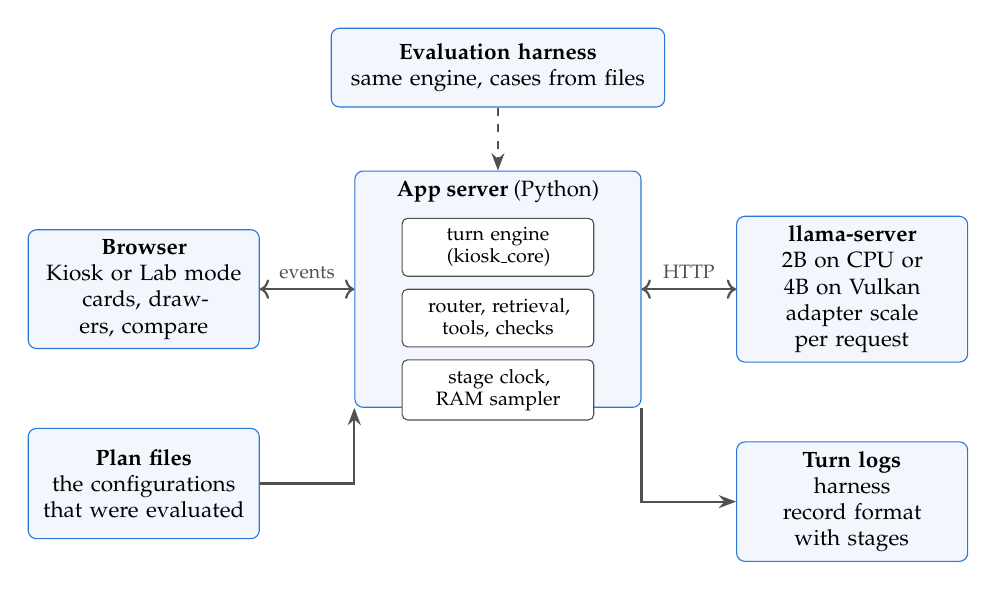
\begin{tikzpicture}[
  node distance=5mm and 7mm,
  box/.style={draw=qblue, fill=boxfill, rounded corners=3pt, align=center, font=\footnotesize, minimum height=14mm,
              text width=27mm},
  sbox/.style={draw=ink2, fill=white, rounded corners=2pt, align=center, font=\scriptsize, text width=22mm,
               minimum height=7mm},
  arr/.style={-{Stealth[length=2.2mm]}, thick, ink2}]
\node[box] (ui) {\textbf{Browser}\\Kiosk or Lab mode\\cards, drawers, compare};
\node[box, right=12mm of ui, text width=34mm, minimum height=30mm] (app) {};
\node[font=\footnotesize, align=center, anchor=north] at (app.north) {\textbf{App server} (Python)};
\node[sbox, below=6mm of app.north] (eng) {turn engine (kiosk\_core)};
\node[sbox, below=1.5mm of eng] (ret) {router, retrieval, tools, checks};
\node[sbox, below=1.5mm of ret] (stg) {stage clock, RAM sampler};
\node[box, right=12mm of app] (llama) {\textbf{llama-server}\\2B on CPU or 4B on Vulkan\\adapter scale per request};
\node[box, below=10mm of ui] (plans) {\textbf{Plan files}\\the configurations\\that were evaluated};
\node[box, below=10mm of llama] (logs) {\textbf{Turn logs}\\harness record format\\with stages};
\node[box, above=8mm of app, text width=40mm, minimum height=10mm] (har) {\textbf{Evaluation harness}\\same engine, cases from files};
\draw[arr, <->] (ui) -- node[above, font=\scriptsize] {events} (app);
\draw[arr, <->] (app) -- node[above, font=\scriptsize] {HTTP} (llama);
\draw[arr] (plans) -| (app.south west);
\draw[arr] (app.south east) |- (logs);
\draw[arr, dashed] (har) -- (app);
\end{tikzpicture}}
\caption{The app on one kiosk machine. The harness and the app call the same turn engine, so they cannot drift apart.}
\label{fig:arch}
\end{figure}

\paragraph{A turn engine shared with the harness.} The turn logic moved out of the harness into a package,
\texttt{kiosk\_core}, behind one call, \texttt{run\_turn(session, message, config, emit)}. The harness passes a no-op
\texttt{emit}; the app forwards each event to the browser. The turn record is the harness's own case record plus a
stage list, so the existing scorers and summaries read live sessions too.

\paragraph{Eight stages.} Every turn is split into input, route, retrieval, harness tools, model rounds (reading and
writing), the model's tool calls, checks and output, with sub-stages for the router, BM25, query encoding, fusion,
re-ranking, each tool call and the answer check. Entering a stage closes the one before, so the stages cover the turn
with no gaps. Each stage records its start, duration, and the memory of llama-server and the app at its end and its peak.

\paragraph{Two memory policies.} \emph{Resident} keeps everything loaded. \emph{Sequential} keeps the query encoder,
re-ranker and router in a worker process that starts at routing and stops at the model's first round, because freeing a
model inside Python does not reliably return its memory to the system. Step~8 chose between them for Tier~A.

\paragraph{The model server manager.} It starts llama-server with the plan's arguments and the tier's build, loads every
adapter of the model at scale~0, and sets the scale per request, so switching the adapter costs no reload. At the user's
request during Step~4, both modes now load and warm the model when the app starts, not on the first message, and a
watchdog reloads llama-server if it stops. The page shows ``Getting ready'' until the model is loaded.

\subsection{The two modes}
Kiosk mode (Figure~\ref{fig:kiosk}) shows only the chat: no sidebar, picker or drawers, and a chat resets after two idle
minutes. Lab mode adds a four-part picker (tier, model, pipeline, adapter). Its pipelines are the rungs of Objective~3's
ablation ladder (Model only, + Retrieval, O3-final, the deployed setup) and a Custom mode with seven switches, each with
an evidence note from the results; a combination with no results is labelled untested. Compare mode runs one message
through two setups in turn, so two models never hold memory at once. The tool-call drawer lists each call, who made it
(model, harness or guard), its arguments and the result as the model saw it. The stage drawer shows a waterfall of the
turn, summary chips and a RAM bar against the tier's budget (Figure~\ref{fig:lab}).

\begin{figure}[H]
\centering
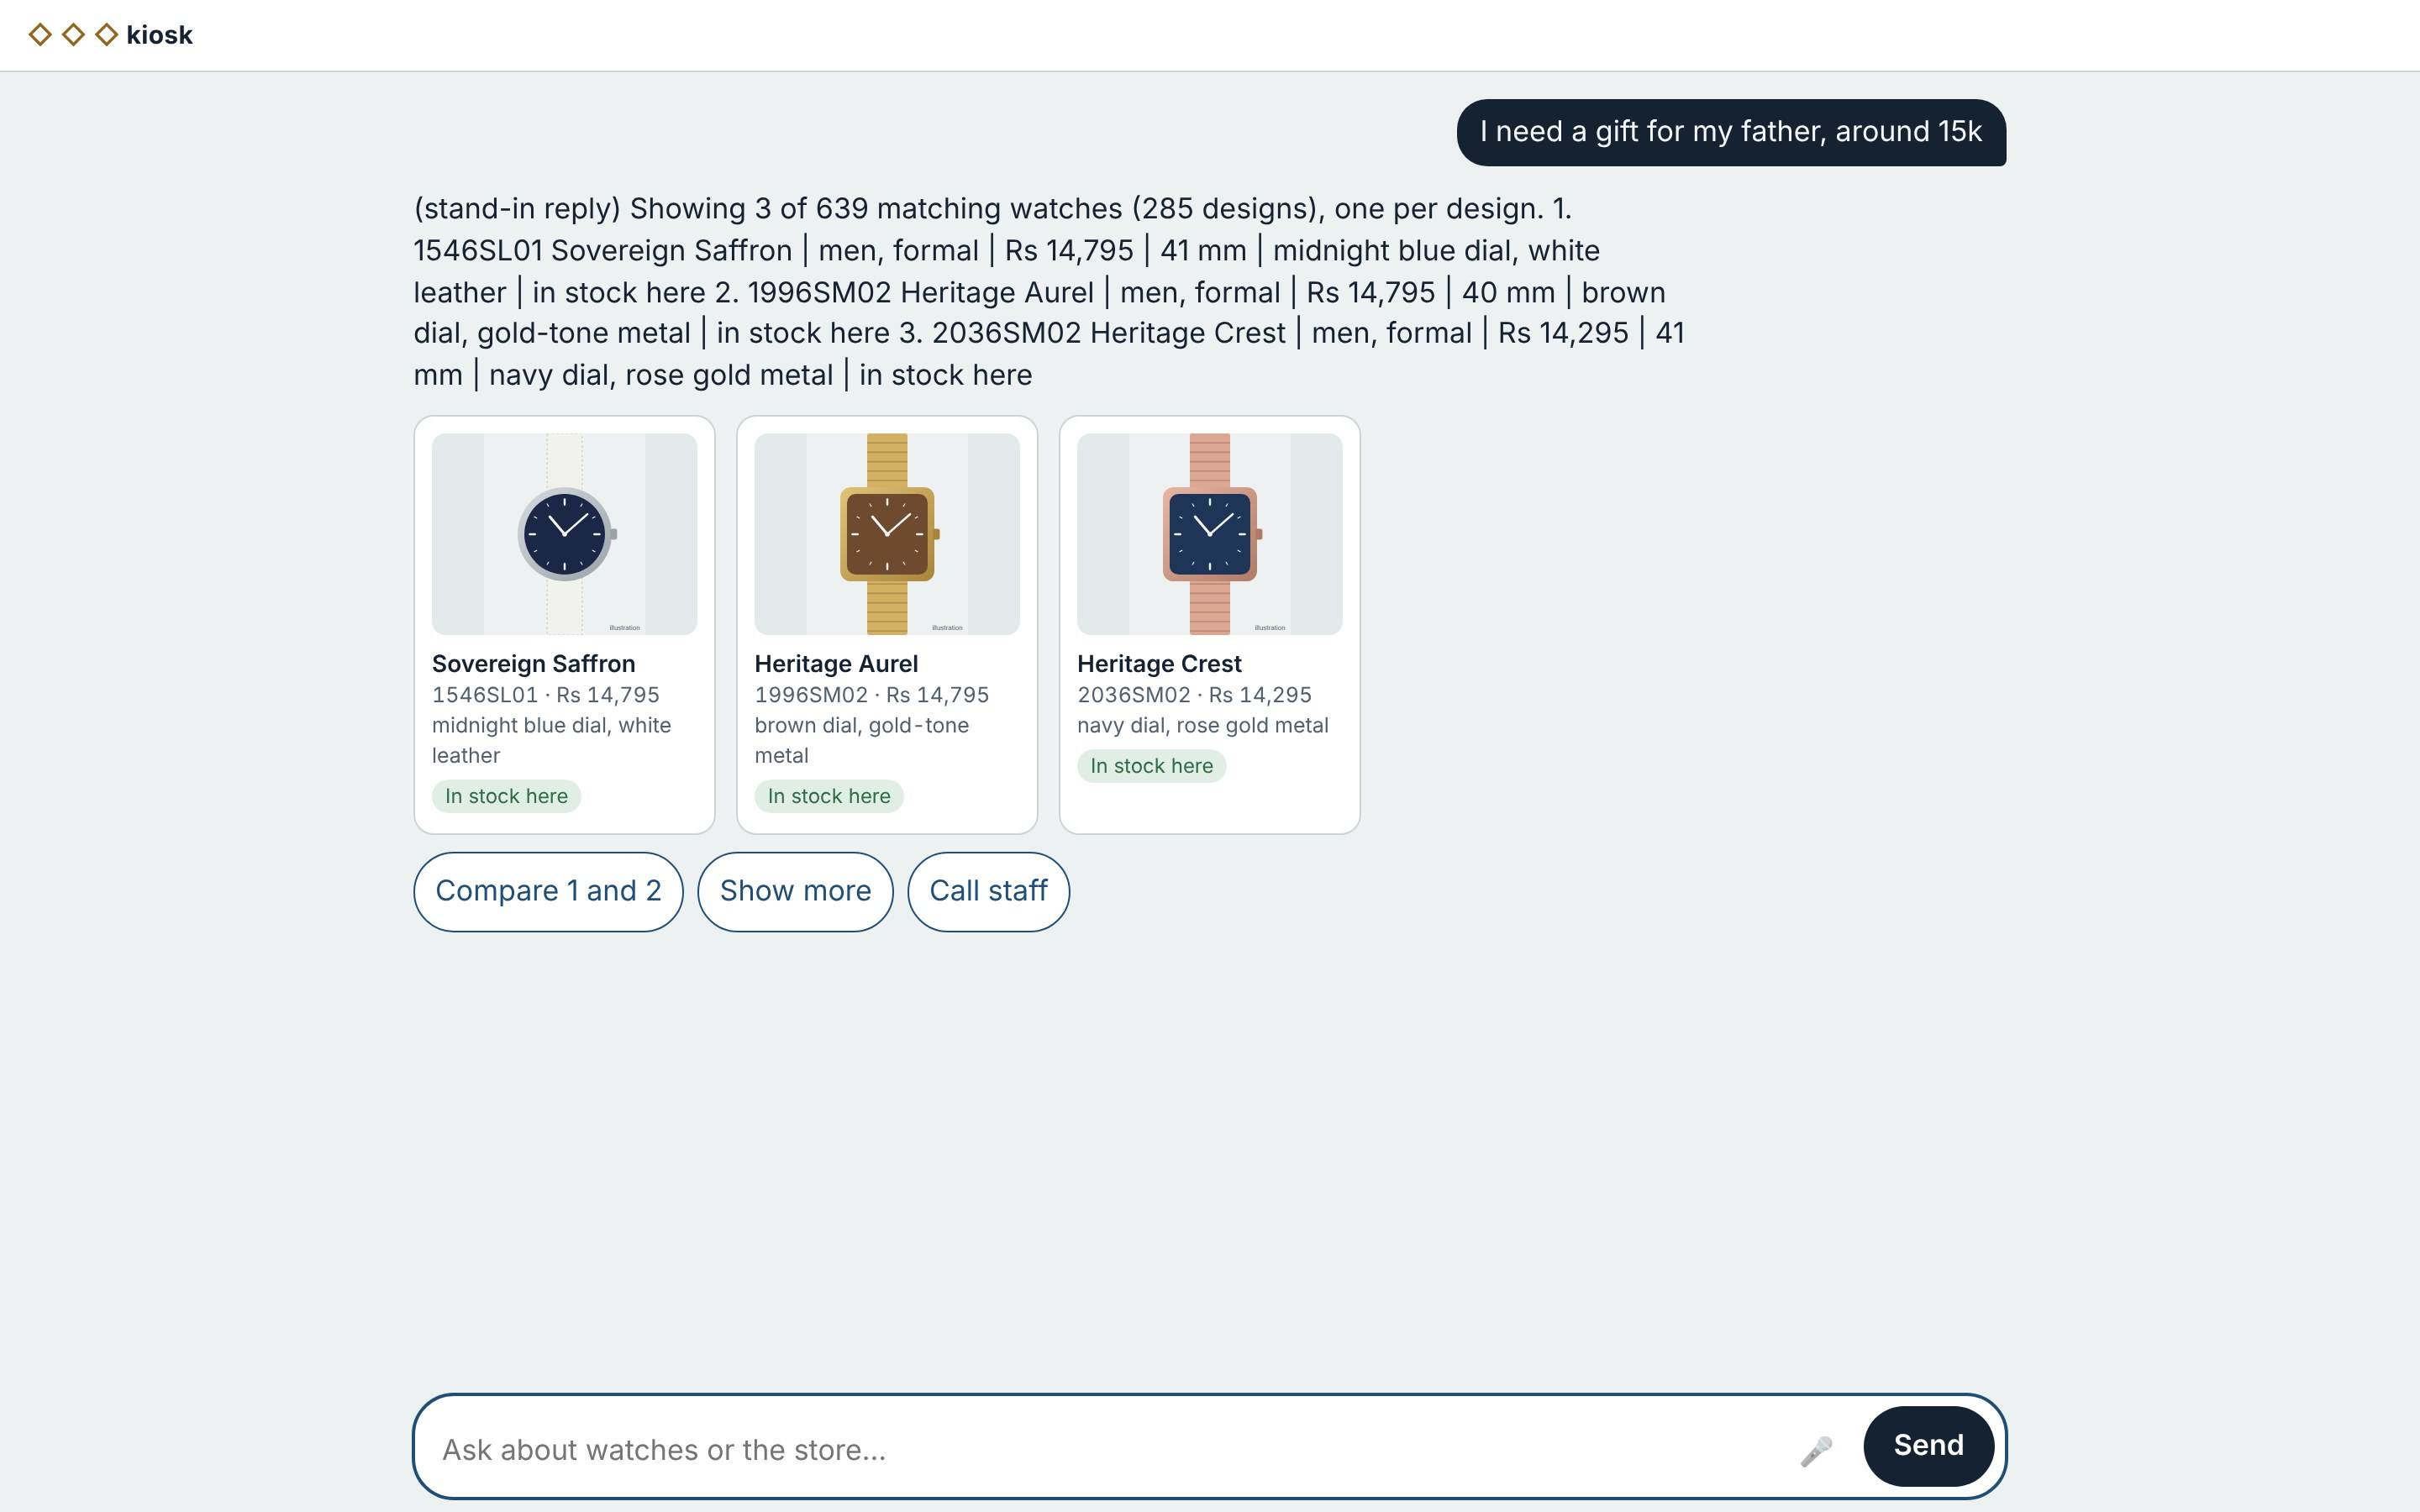
\includegraphics[width=0.86\textwidth]{figs/shot_kiosk_shopping.jpg}
\caption{Kiosk mode after a shopping question, with image cards and quick replies. Screenshot with the stand-in model
server used for interface tests; reply text from the real models is in Section~\ref{sec:walk}.}
\label{fig:kiosk}
\end{figure}

\begin{figure}[H]
\centering
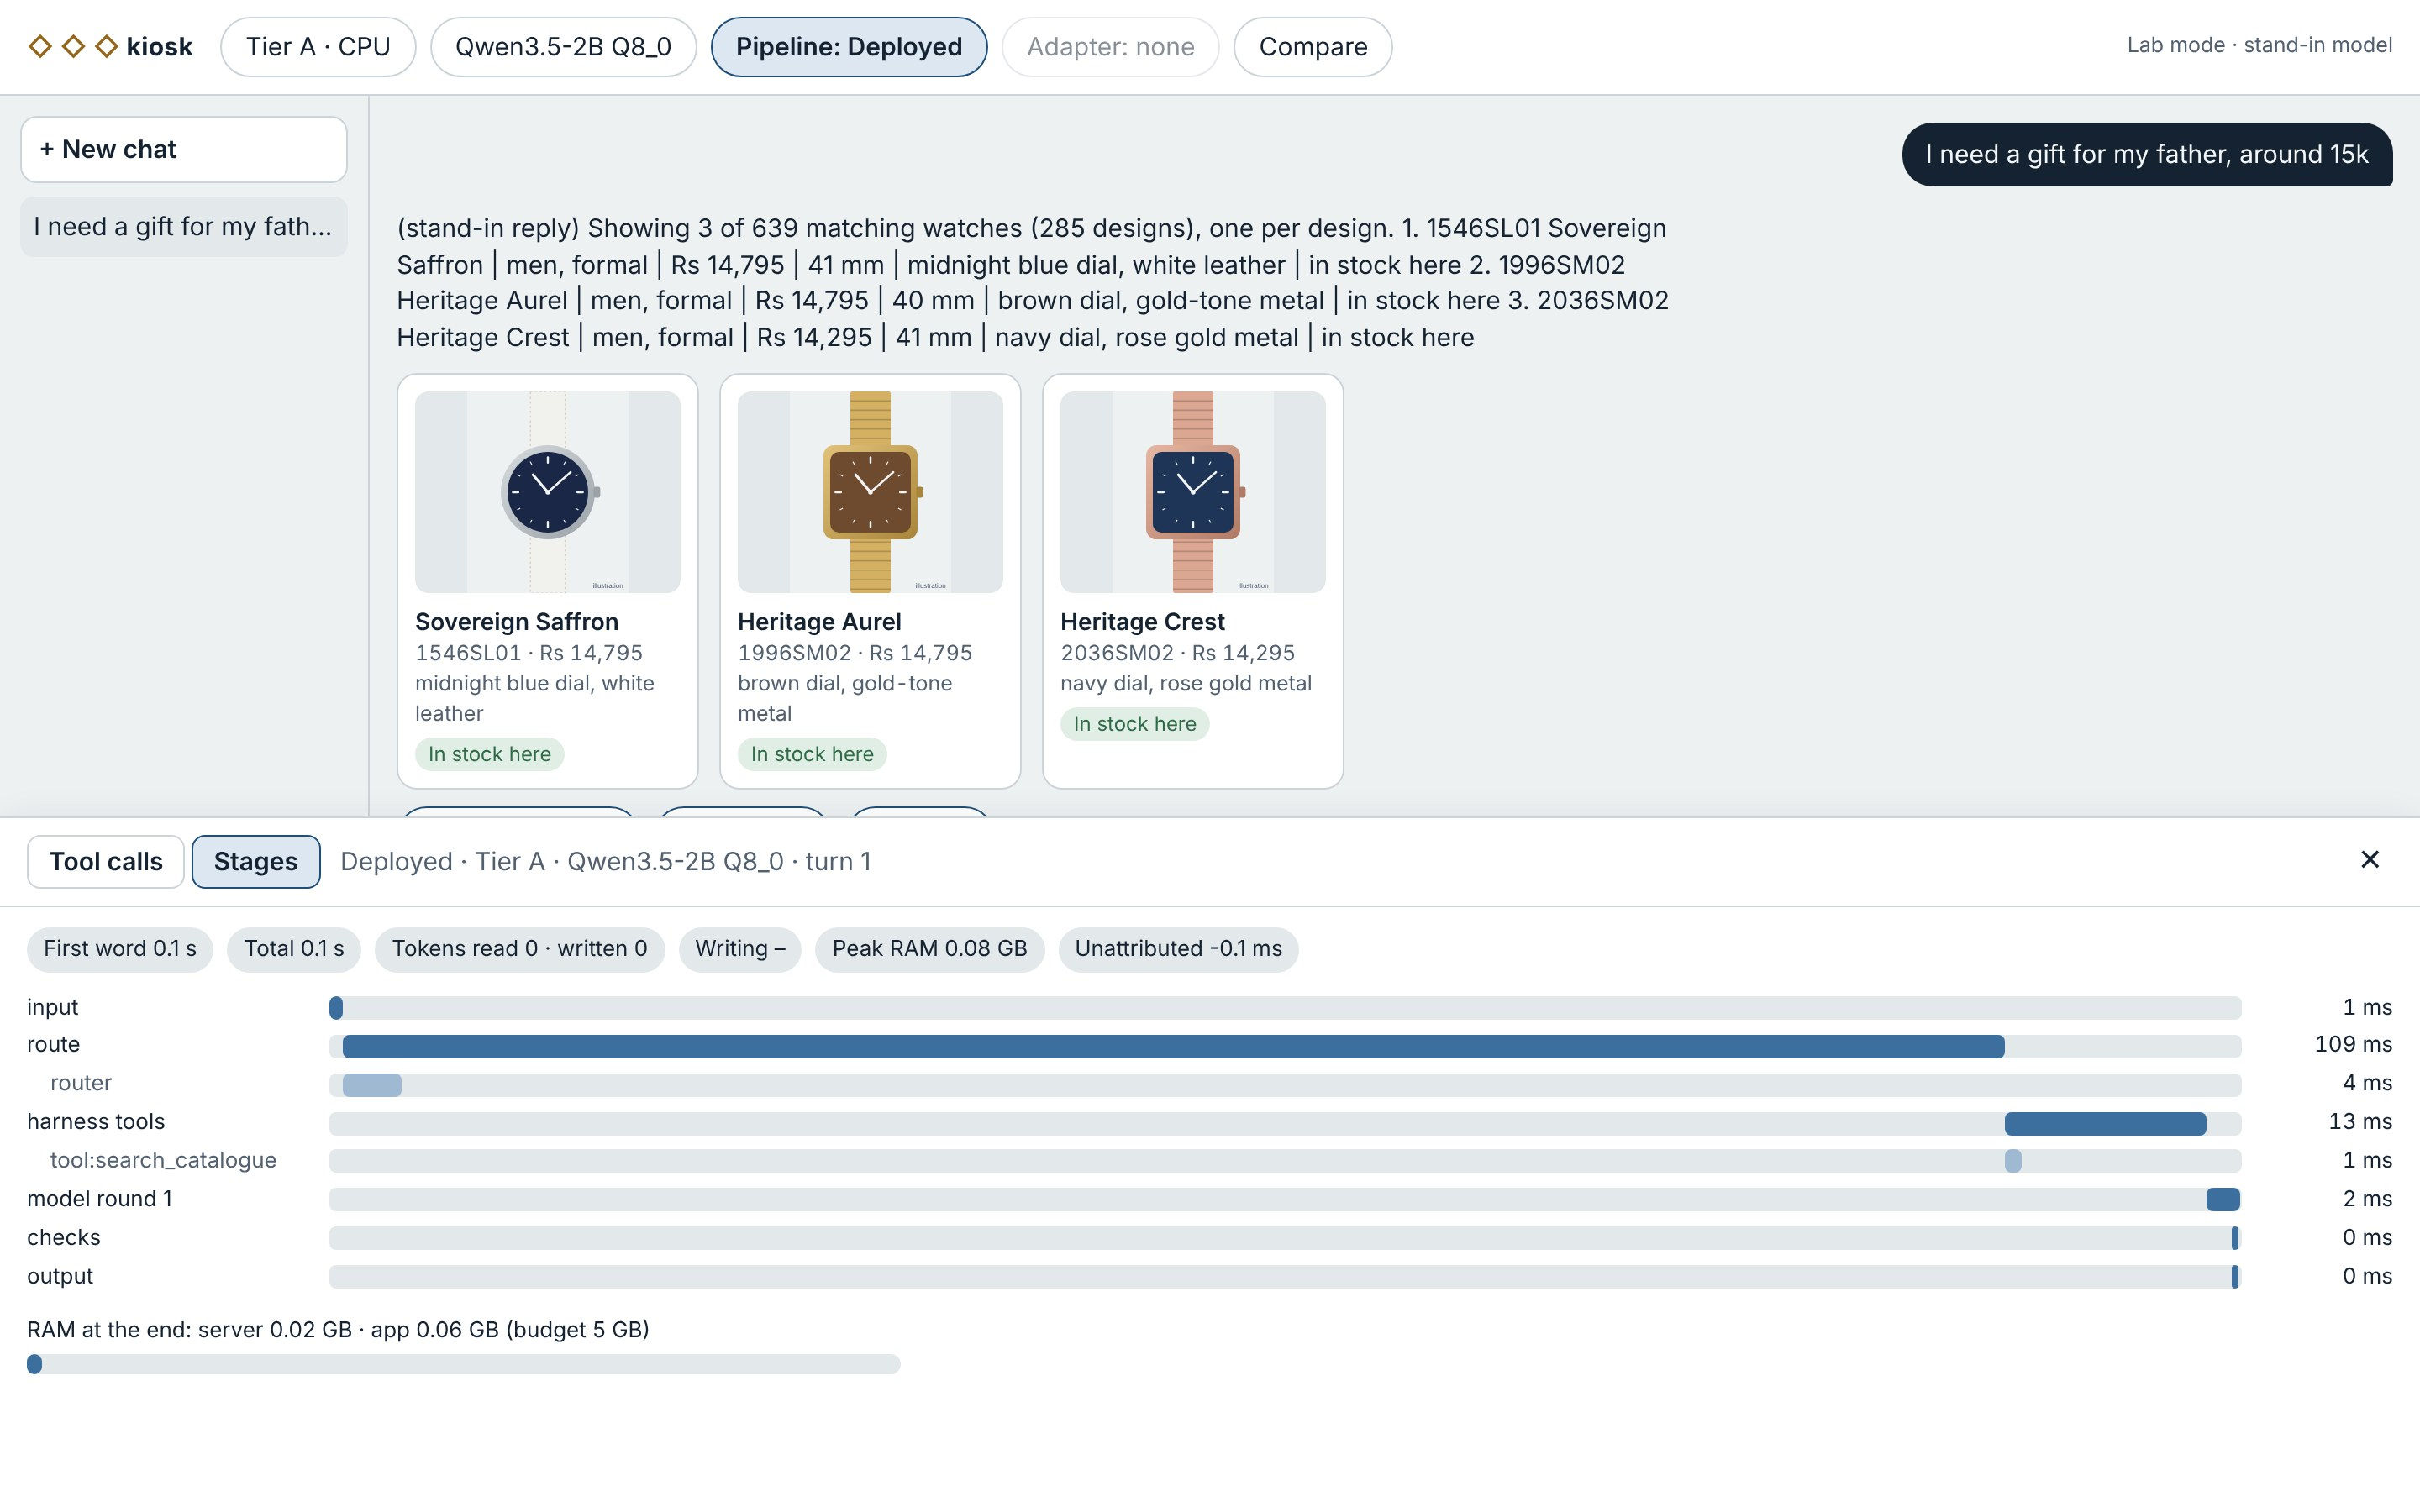
\includegraphics[width=0.49\textwidth]{figs/shot_lab_stages.jpg}\hfill
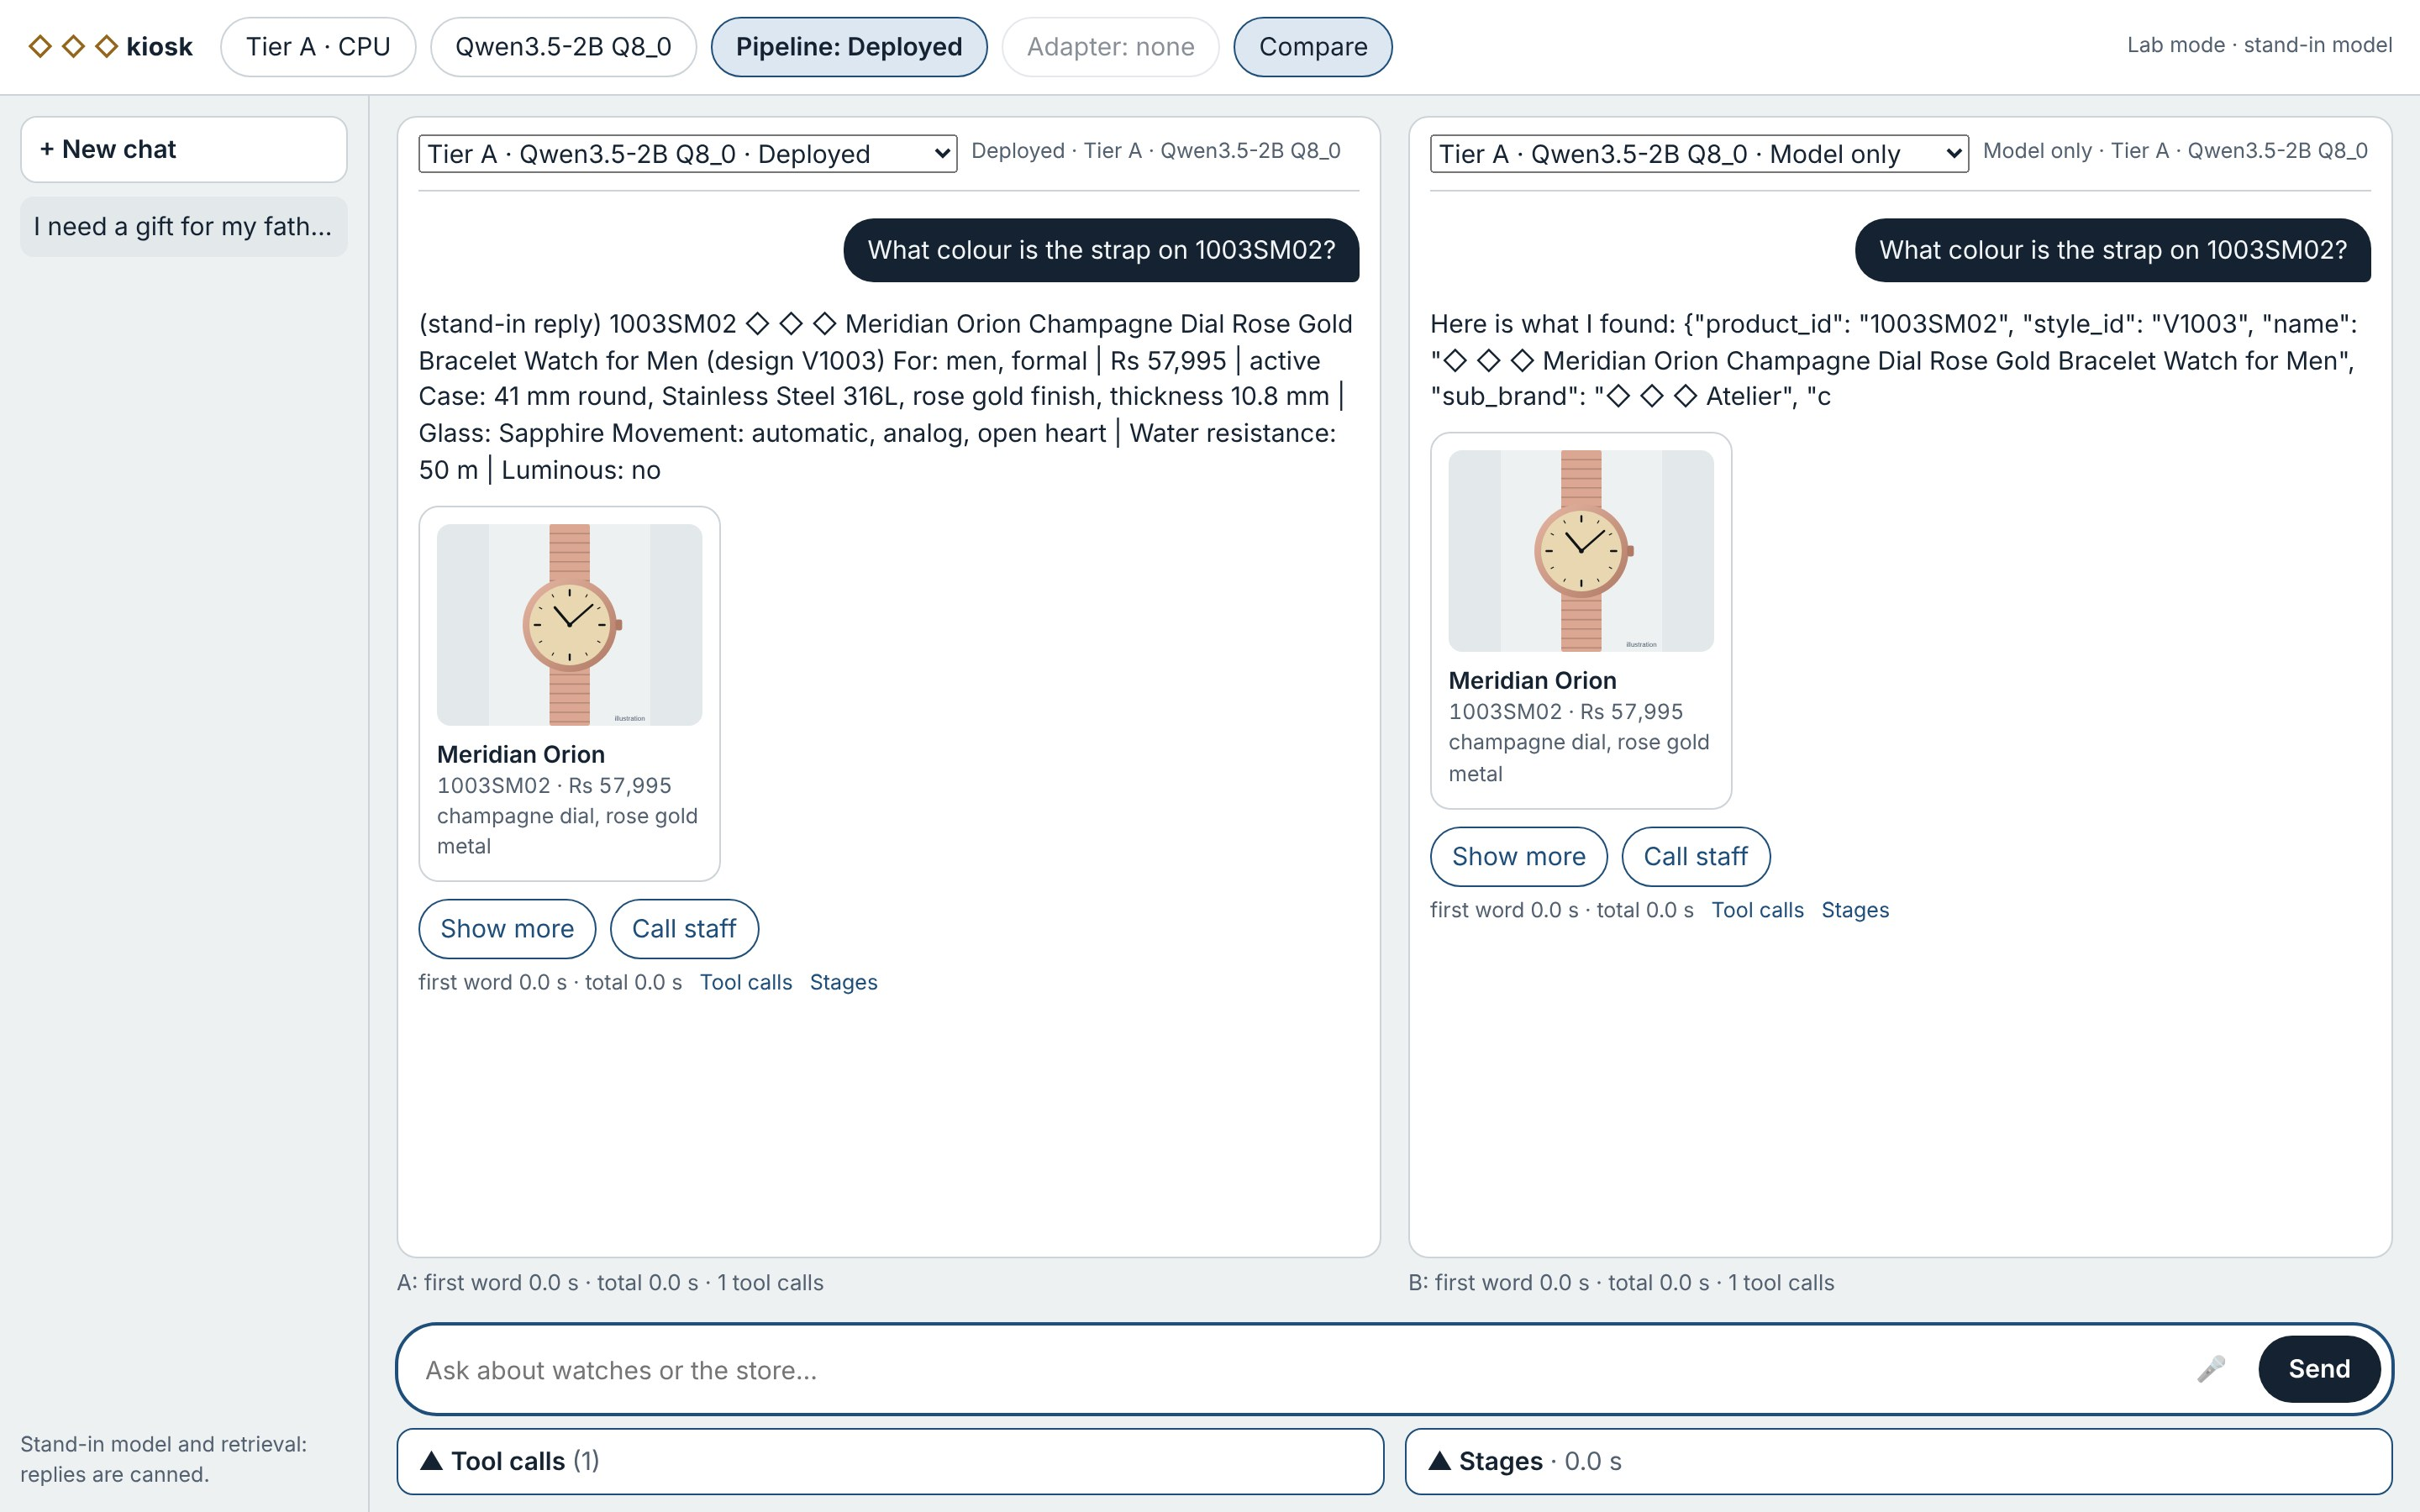
\includegraphics[width=0.49\textwidth]{figs/shot_lab_compare.jpg}
\caption{Lab mode with the stand-in model server. Left: the stage drawer for a shopping turn. Right: compare mode, the
deployed setup against the bare model on the same question.}
\label{fig:lab}
\end{figure}

\subsection{Product images}
The catalogue had no images. Following common retail practice, images are held apart from the product record and linked
by SKU, with one main image and further views per SKU and file names in the GS1 style, from each SKU's GTIN-14 and a
view code~\cite{gs1}. A media table (\texttt{data/kiosk/media.csv}) lists 4,554 illustrations: front, side and back for
each of the 1,518 SKUs, drawn by a generator from the SKU's own case shape, finish, dial and strap, and labelled as
illustrations. Images reach the chat in two ways. Cards are attached by the engine for products the reply names and this
turn's tools returned, so the model never chooses a picture. Explicit requests (``show me the back of it'', ``photo
dikhao'') are routed to a \texttt{show\_product\_images} tool run by the kiosk for the watch in focus
(Figure~\ref{fig:images}). Any URL in model text is removed.

\begin{figure}[H]
\centering
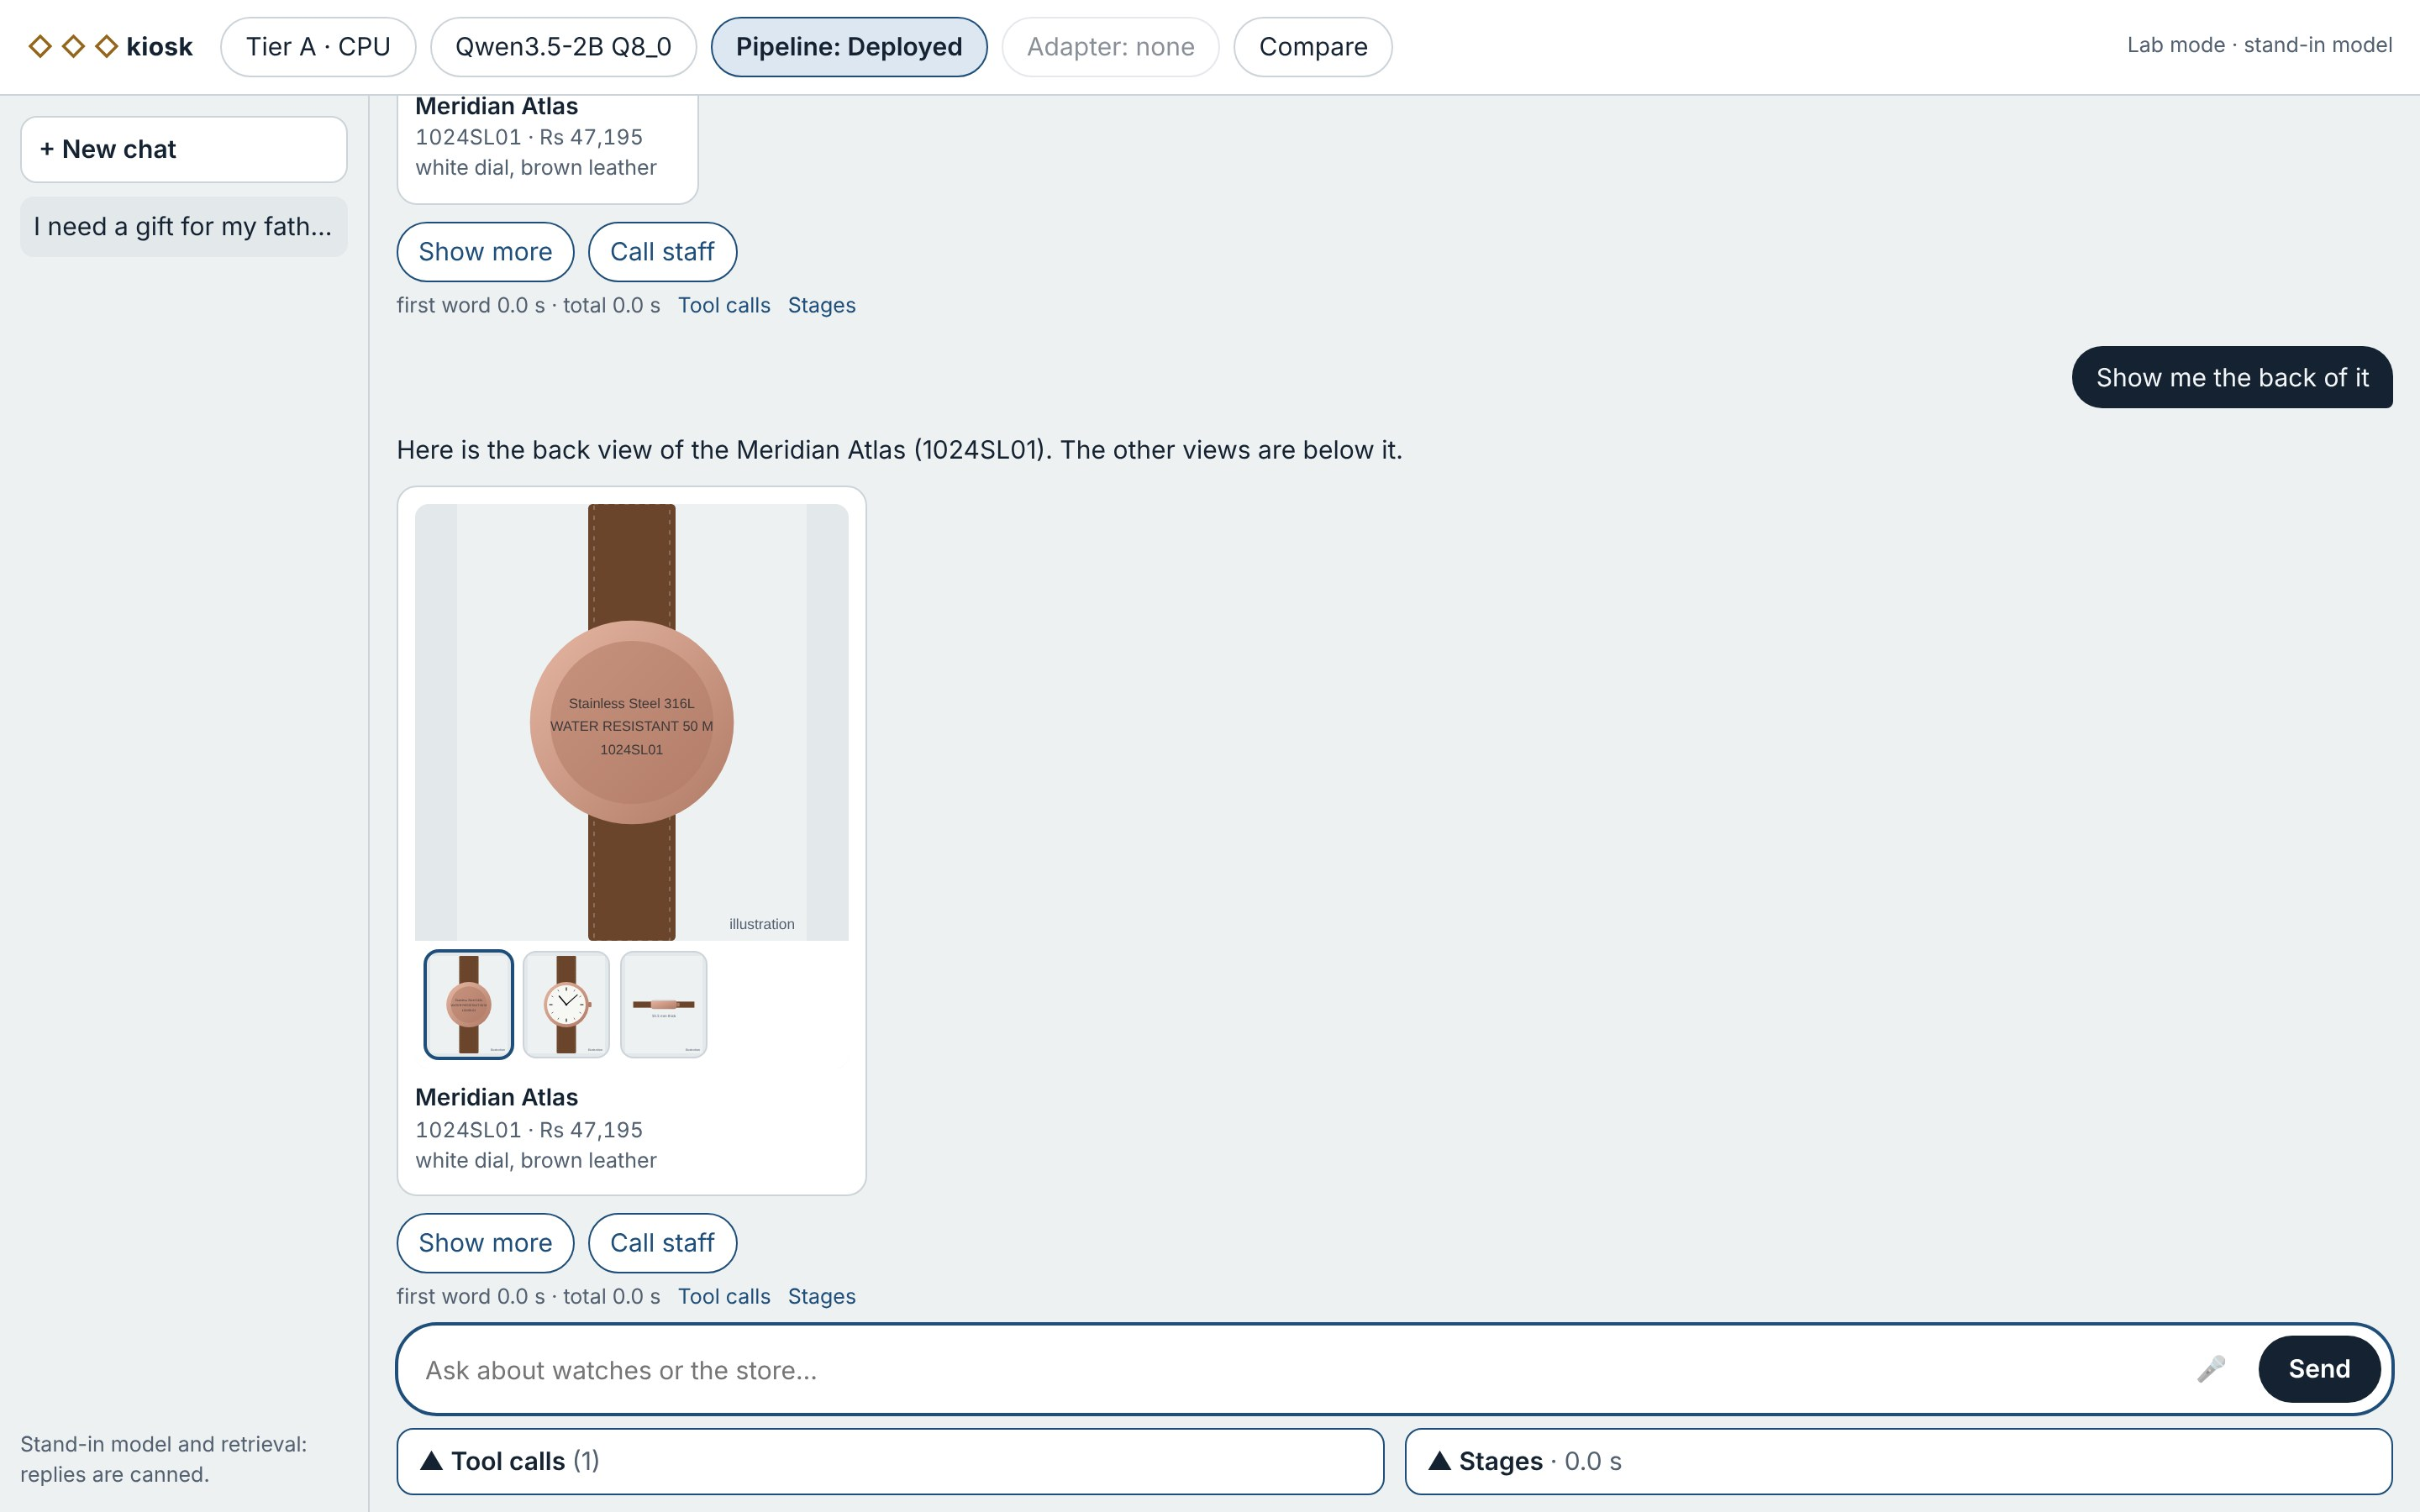
\includegraphics[width=0.62\textwidth]{figs/shot_lab_images.jpg}
\caption{``Show me the back of it'': the back view first, the other views below (stand-in model server).}
\label{fig:images}
\end{figure}

\subsection{Packaging and offline operation}
A package builder writes one folder per tier with the code, data, llama-server, the model file, start scripts, an
operator's guide and a manifest of every file's checksum. The deployed setup reads a few result files (fallback
thresholds, the re-ranker choice, the retrieval depth); if one is missing the build stops, so the package can never fall
back to a default silently. The start script runs a launcher that starts the app offline, opens the browser full-screen,
and restarts the app if it stops. In offline mode every app process refuses, and logs, any connection that would leave
the machine.

\subsection{Deviations from the design}
\begin{itemize}
  \item \textbf{Backend:} Python's standard-library HTTP server instead of FastAPI, so the kiosk needs nothing installed
        beyond the project's environment. The API and events are as designed.
  \item \textbf{Frontend:} plain JavaScript with no build step instead of React with TypeScript, so no Node toolchain is
        needed. It can be ported later without changing the API.
  \item \textbf{Sessions} are kept in memory, without the planned SQLite copy; turn logs are written as designed.
  \item \textbf{Images} are vector illustrations, so the derived raster sizes were not built; real photos will need them.
  \item \textbf{Start-up} uses a batch file and a Python launcher instead of a PowerShell script.
  \item \textbf{Staff calls} are confirmed in the reply text; the planned confirmation card with the ticket number was not
        built.
\end{itemize}

% ===========================================================================
\section{Method}\label{sec:method}
% ===========================================================================
As in the earlier objectives, each step's rule was written into the objectives document before its run, and any deviation
is stated where it happened. All runs are on the same laptop (Intel Core i5-1240P, 16\,GB RAM, Intel Iris Xe graphics,
Windows~11) with the models of Objectives~1--4, unchanged. The app, engine, tests and measurement scripts were written
for this project; an AI coding assistant helped write and debug parts of this code. Table~\ref{tab:steps} lists the
steps.

\begin{table}[H]
\centering\small
\caption{The ten steps of Objective~5 and their rules.}\label{tab:steps}
\begin{tabularx}{\textwidth}{p{0.5cm} p{3.4cm} L}
\toprule
Step & Builds & Rule (fixed before the run) \\
\midrule
1 & Design & Reviewed \\
2 & Shared turn engine & O3-final, both models, Vulkan, temperature 0; 40 store questions, 30 tool cases, 10 dialogues
(dev); old code and new engine in the same sitting; $\ge$95\% identical, every difference traced \\
3 & Stages, stage manager & Tier~A, CPU, dev speed subset, 2 repeats, clock off and on alternating: every turn complete;
stages within $\max(5\%, 5\,\text{ms})$ of the total in $\ge$99\% of turns; clock adds $\le$50\,ms to the median \\
4 & API, model server, streaming & Streamed and non-streamed requests parse identically on all 30 tool cases $\to$ every
round streams; real-model smoke tests \\
5 & Chat UI & Browser tests of the scenarios on the stand-in; axe-core~\cite{axe}: no serious or critical issue \\
6 & Compare mode & 10 dev cases (5 store, 5 tool): each compare column equals the same setup run alone \\
7 & Images & 40 dev and 40 test image requests (half Hinglish, a quarter follow-ups), both models: right SKU and view
$\ge$95\%; no wrong-SKU image; cards match named products on every dev reply; lookup p95 $\le$50\,ms; test used once \\
8 & In-place measurement & Each tier's deployed setup through the app, alternating with the harness on the same cases;
dev speed subset ($\times 2$), then the test speed subset ($\times 1$); Tier~A policy: the lower median total if within
5\,GB \\
9 & Walkthrough & The six design scenarios, Kiosk mode (compare in Lab mode), both tiers, each passed or failed with its
trace kept \\
10 & Packaging, offline & From the package, network off: the walkthrough again, plus restarts, no network use, and the
same replies as the project \\
\bottomrule
\end{tabularx}
\end{table}

\paragraph{The six scenarios and their checks.} The walkthrough script starts the app itself and talks to it through its
API, as a browser would. Its pass rules were written into the script before the run:
\begin{enumerate}[label=\arabic*.]
  \item \textbf{Shopping.} ``I need a gift for my father, around 15k'': at most two slot questions, then 1--3 cards with
        code, name, price and image, all from this turn's catalogue results; then ``Is the second one in stock here?'':
        a stock check on the second watch the reply named, and a reply that agrees with it.
  \item \textbf{Store question.} ``What does the warranty cover?'': retrieval ran, and the reply passed the answer check
        or is the fixed decline.
  \item \textbf{Hinglish.} After ``Tell me about 1024SL01'' (brown strap; its design has a black-strap variant,
        1024SL03): ``Kya ye black strap mein milta hai?'' The reply is Hinglish and says the black variant exists.
  \item \textbf{Images.} ``Show me the back of it'': the back view of a variant of that design first, every picture of
        one SKU.
  \item \textbf{Compare (Lab).} ``What colour is the strap on 1003SM02?'' to O3-final and to the bare model: both
        columns finish with a full stage list, and O3-final says rose gold or declines.
  \item \textbf{Hand-off.} ``Can someone help me try it on?'': a staff call for a try-on returns a ticket, the reply says
        someone is coming, and the ticket is in the staff log.
\end{enumerate}
Two further checks run on every turn: no error event and a non-empty reply, and the brand name never reaches the browser.
A Kiosk-lock check confirms that Kiosk mode refuses a setup change and compare. Step~10 adds four more:
\textbf{R1}, llama-server is killed and must come back by itself; \textbf{R2}, the app is killed and the launcher must
bring it back, both within twice the load time plus 60\,s; \textbf{N}, no connection attempt leaves the machine; and
\textbf{P}, scenarios 1--5 give the same replies from the package as from the project in Step~9.

% ===========================================================================
\section{Results}\label{sec:results}
% ===========================================================================

\subsection{Step 2: the app runs what was evaluated}
The first parity run matched on 125 of 160 cases (78.1\%), against the 95\% rule. Every difference was traced to one
cause. All 34 differing store questions and the one differing tool case came from the 2B's new-engine run: 33 had
the same prompt and a different model output, and two lost their connection to the server. A llama-server left running from an Objective~4 session, with its adapter
loaded, still held the port, so the new-engine run talked to the wrong server. The plan runner now checks that the port
is free before it starts a server and confirms the adapters it loaded. On the rerun, \textbf{160 of 160} cases were
identical in reply and tool calls: \met.

\subsection{Step 3: every stage measured, at no cost}
All 160 turns logged every stage, and in 160 of 160 the stages added up to the turn's total within the tolerance:
\met. With the clock on, the median total changed by $-746$\,ms on store questions (95\% interval $[-993, -402]$) and
$-12$\,ms on tool cases ($[-75, -1]$): \met. These are drift on the laptop between alternating runs; the clock's own
measured cost is 0.1--0.2\,ms per turn. The sequential policy's worker took 1.8--1.9\,s to start at each turn
(reported; Step~8 decides).

\subsection{Step 4: streaming and the real models}
Each model request was sent both streamed and non-streamed. The two were identical on all 30 tool cases for both
models (2B: 6 tool-enabled requests and 19 final rounds; 4B: 10 and 38), so \textbf{every model round streams}. The app
releases text only at word boundaries and holds back anything that could be the start of a tool call. Smoke tests with
the real models passed five API scenarios on both tiers. The first word of the 2B's shopping reply came only after
27.5\,s, because warm-up had not prepared the variant of the request with tools switched off; after the warm-up was
fixed, the same turn's first word came at 3.5--4.0\,s in Steps~9 and~10.

\subsection{Step 5: interface and accessibility}
The UI passed its browser tests on the stand-in model server. The axe-core scan of nine states in both modes found
\textbf{no serious or critical issue} (\met). It found one moderate issue, a page with no level-one heading, which was
fixed. A built-in keyboard check found that the message box showed no visible focus, which was also fixed. The colour
scheme was reworked to a dark-navy and brass palette with a dark mode, checked to WCAG AA contrast.

\subsection{Step 6: compare mode}
On the first run, 39 of 40 compare columns equalled the same setup run alone. The one difference was a staff hand-off
(HND-020) on Tier~B. Staff tickets are numbered across chats, so the compare column and the single run were given
different ticket numbers, and the model reads the number. Masking the number did not help, because it changes the
prompt, not only the reply. Lab mode can now set the next ticket number, so a single run gets the ticket its column got.
With that, HND-020 matched in both columns: \met. Only that case was rerun.

\subsection{Step 7: product images}
On dev and then once on test, \textbf{80 of 80} image requests (40 cases, both models) showed the right SKU and view, in
English and Hinglish and for codes, design names, follow-ups and requests that are not about pictures. No reply showed a
picture of a different SKU, all 186 cards matched the products their reply named, and the lookup's p95 was 0.005\,ms:
all four targets \met. Two faults were fixed on dev before the test run: ``see-through caseback'' and a bare
``caseback'' had been read as requests for a picture. The test cases had been run once before, on the stand-in model,
while the scorer was being checked; their real-model run here is the first and only one.

\subsection{Step 8: the app adds almost nothing}\label{sec:speed}
Each tier's deployed setup ran through the app's API, alternating case by case with the harness on the same cases
(Figure~\ref{fig:latency} and Table~\ref{tab:speed}). The app's overhead was \textbf{0.4\% or less} of the median total
and \textbf{0.02\,s or less} on the first word in every run (Figure~\ref{fig:overhead}), and all 556 replies through the
app equalled the harness's. On Tier~A, the resident policy had the lower median total (7.58\,s against 7.94\,s) and
peaked at 3.21\,GB, so \textbf{resident was chosen}. Sequential saves only 0.23\,GB, and its worker adds 1.6\,s to
routing (Figure~\ref{fig:policy}). Both tiers peak below Objective~2's measurements (Figure~\ref{fig:ram}).

\begin{figure}[H]
\centering
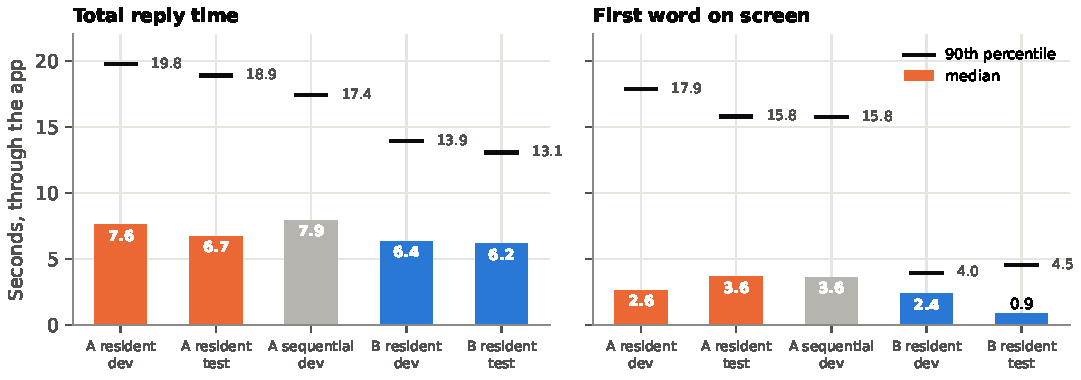
\includegraphics[width=\textwidth]{figs/fig_latency.pdf}
\caption{Reply times through the app: medians (bars) and 90th percentiles (ticks). Dev runs have 70 cases and 2
repeats; test runs 68 cases and 1 repeat.}
\label{fig:latency}
\end{figure}

\begin{table}[H]
\centering\small
\caption{In-place measurement (seconds, medians over cases). Overhead is the median of per-case differences, app minus
harness.}\label{tab:speed}
\setlength{\tabcolsep}{4pt}
\begin{tabularx}{\textwidth}{L r r r r r r}
\toprule
Run & \shortstack[r]{Total\\p50 / p90} & \shortstack[r]{First word\\p50 / p90} & \shortstack[r]{Overhead\\(total)} &
\shortstack[r]{Writing\\tok/s} & \shortstack[r]{Peak\\RAM} & \shortstack[r]{Same\\reply} \\
\midrule
A resident, dev & 7.58 / 19.78 & 2.63 / 17.88 & +0.03 (0.4\%) & 15.4 & 3.21\,GB & 140/140 \\
A resident, test & 6.74 / 18.90 & 3.64 / 15.80 & +0.01 (0.2\%) & 15.1 & 3.16\,GB & 68/68 \\
A sequential, dev & 7.94 / 17.41 & 3.62 / 15.76 & $-$0.01 ($-$0.1\%) & 17.0 & 2.98\,GB & 140/140 \\
B resident, dev & 6.36 / 13.94 & 2.38 / 3.95 & +0.01 (0.1\%) & 9.6 & 4.76\,GB & 140/140 \\
B resident, test & 6.16 / 13.06 & 0.89 / 4.54 & +0.02 (0.4\%) & 9.7 & 4.74\,GB & 68/68 \\
\bottomrule
\end{tabularx}
\end{table}

\begin{figure}[H]
\centering
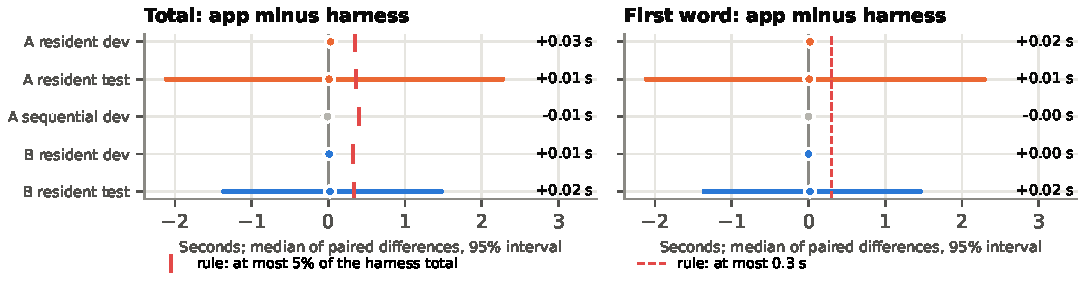
\includegraphics[width=\textwidth]{figs/fig_overhead.pdf}
\caption{App overhead against the harness. The test runs have one repeat, so their intervals are wide; the rules apply to
the medians, which meet them in every run.}
\label{fig:overhead}
\end{figure}

\begin{figure}[H]
\centering
\begin{minipage}{0.58\textwidth}\centering
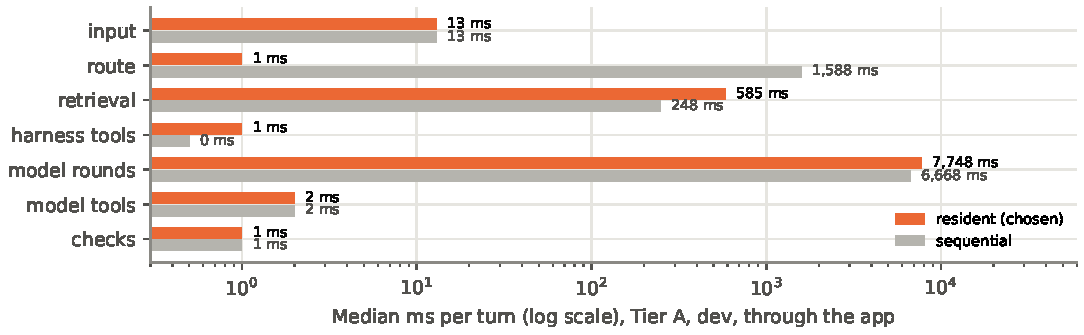
\includegraphics[width=\textwidth]{figs/fig_policy.pdf}
\caption{Tier~A per stage under each policy.}\label{fig:policy}
\end{minipage}\hfill
\begin{minipage}{0.40\textwidth}\centering
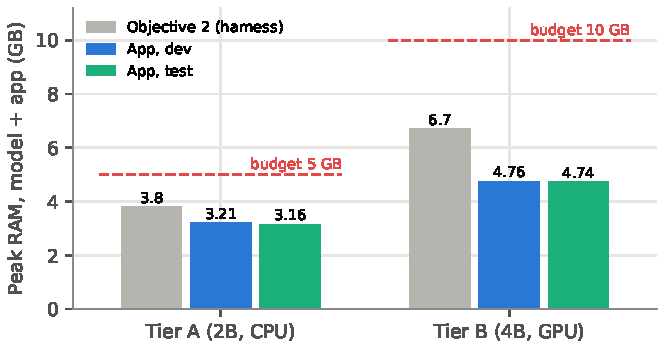
\includegraphics[width=\textwidth]{figs/fig_ram.pdf}
\caption{Peak RAM against budget.}\label{fig:ram}
\end{minipage}
\end{figure}

Two patterns stand out. First, \textbf{Tier~A's slow tail is store questions}: their first word comes at 7.3\,s
(median, dev) against 2.0\,s for tool cases, because the 2B often takes more than one model round before it answers.
That gives the 90th percentile of 16--18\,s. Second, \textbf{resident retrieval took 585\,ms through the app} against
278\,ms in Step~3 and 248\,ms under the sequential policy. The likely cause is the retrieval models competing with
llama-server for the four CPU cores; it was not investigated, and it does not change the policy choice.

\subsection{Step 9: the walkthrough}\label{sec:walk}
On the first run both tiers passed six of seven checks, and scenario~3 (Hinglish) failed on both
(Figure~\ref{fig:walk}). The 2B answered in English and listed only brown and grey straps. The 4B answered in Hinglish
that the watch on screen (1024SL01) has no black strap, without saying that its design comes in one. The cause was in the
kiosk, not the models: ``milta hai'' was not on the list of colour-question phrases, so the question went down the
store-information path instead of the stock path, where the kiosk looks up every variant of the design. The phrases
``milta hai'', ``aata hai'' and ``strap mein'' were added. Of all customer messages in the evaluation sets, eight change
how they are classified, and none is a follow-up with a watch in focus, so no earlier result changes. A dry run on the
stand-in had found a second gap before the real run: ``the second one'' named no watch. The kiosk now resolves a place in
its own last list, in English and Hinglish (``doosra wala''); no evaluation message uses such a phrase.

On the rerun of scenarios 3, 4 and 6, \textbf{the 2B passed}: ``Haan, 1024SL03 Meridian Atlas black strap mein
available hai.'' \textbf{The 4B failed again}: ``Nahi, 1024SL01 mein black strap nahi milta. Ye sirf brown leather strap
wala hai.'' Table~\ref{tab:walk} gives the real replies. Every other scenario passed on both tiers. In the shopping
scenario, ``the second one'' reached the stock check on the right watch. The hand-off called staff and logged the
ticket. The store answer passed the answer check. In the compare scenario, the bare model did not invent a colour, as the
design expected: Model only still has the tools, and it looked the watch up.

\begin{table}[H]
\centering\footnotesize
\caption{Kiosk replies in the Step~10 walkthrough (offline, from the package), shortened. First word and total in
seconds.}\label{tab:walk}
\begin{tabularx}{\textwidth}{p{3.0cm} p{0.4cm} L r r}
\toprule
Customer & Tier & Kiosk & First & Total \\
\midrule
\multirow{2}{3.0cm}{I need a gift for my father, around 15k} & A & Here are 3 men's watches under Rs 15,000: 1.
1546SL01 Sovereign Saffron \ldots & 3.5 & 10.6 \\
 & B & Here are three options for your father under 15k: 1. 1546SL01 Sovereign Saffron / Rs 14,795 \ldots & 3.5 &
17.2 \\
\multirow{2}{3.0cm}{Is the second one in stock here?} & A & Yes, the 1996SM02 Heritage Aurel is in stock here.
\ldots & 4.0 & 6.7 \\
 & B & Yes, the 1996SM02 Heritage Aurel is in stock here. We have one on display and two in the back room. \ldots & 4.9
& 10.7 \\
\multirow{2}{3.0cm}{What does the warranty cover?} & A & Based on the store information, the warranty covers:
manufacturing defects in the movement and battery \ldots & 16.5 & 23.8 \\
 & B & The warranty covers manufacturing defects in the movement and battery. It does not cover straps, glass breakage
\ldots & 5.3 & 9.2 \\
\multirow{2}{3.0cm}{Kya ye black strap mein milta hai?} & A & Haan, 1024SL03 Meridian Atlas black strap mein available
hai. Iska price \textcolor{qred}{Rs 1,29,990} hai. & 4.0 & 6.0 \\
 & B & \textcolor{qred}{Nahi, 1024SL01 mein black strap nahi milta.} Ye sirf brown leather strap wala hai. \ldots & 4.4 &
9.3 \\
\multirow{2}{3.0cm}{Show me the back of it} & A & Here is the back view of the Meridian Atlas (1024SL03). The other
views are below it. & 0.0 & 0.0 \\
 & B & Here is the back view of the Meridian Atlas (1024SL01). \ldots & 0.0 & 0.0 \\
\multirow{2}{3.0cm}{Can someone help me try it on?} & A & Staff has been notified and will come to the kiosk in about 3
minutes to help you try it on. & 2.8 & 4.2 \\
 & B & I have asked a staff member to come and help you. They will be with you in a few minutes. & 4.1 & 6.7 \\
\bottomrule
\end{tabularx}
\end{table}

\begin{figure}[H]
\centering
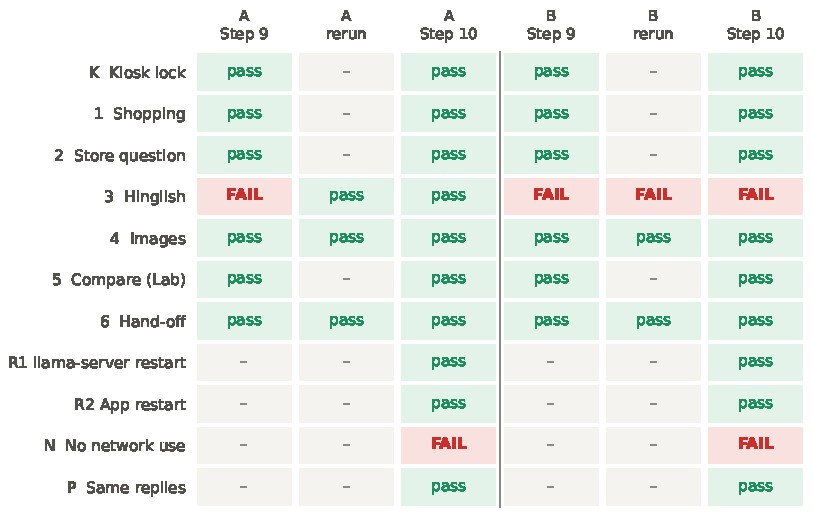
\includegraphics[width=0.72\textwidth]{figs/fig_walk.pdf}
\caption{Walkthrough checks per run. ``Rerun'' repeats scenarios 3, 4 and 6 (one chat) after the colour-phrase fix.
Step~10 runs everything again offline from the package and adds R1, R2, N and P.}
\label{fig:walk}
\end{figure}

\subsection{Step 10: the package, offline}
Each tier's package was built, checked against its manifest, and run with the network off. Kiosk mode was ready
81.8\,s (Tier~A) and 96.6\,s (Tier~B) after the start. Tier~A passed 10 of 11 checks and Tier~B 9 of 11
(Figure~\ref{fig:walk}).
\begin{itemize}
  \item \textbf{Restarts (R1, R2): passed.} With llama-server killed, the app's watchdog reloaded it and the kiosk
        answered again after 35.6\,s (A) and 46.2\,s (B). With the app killed, the launcher restarted it and the kiosk
        answered after 103.0\,s and 103.6\,s, within the limits of 223\,s and 253\,s.
  \item \textbf{Same replies (P): passed.} All eight replies compared, from scenarios 1--5, were identical to the
        project's Step~9 run, so the package behaves like the project.
  \item \textbf{No network use (N): failed.} Each tier's run logged three connection attempts to
        \path{www.google-analytics.com}. The offline guard refused them, so nothing left the machine. There were three
        app starts per run (the kiosk, its restart in R2, and Lab mode), which points to a library sending usage
        telemetry once at start-up. The guard's log records where each attempt came from; that record has not yet been
        examined.
  \item \textbf{Scenario 3} failed again on Tier~B, with the same reply as in Step~9.
\end{itemize}

% ===========================================================================
\section{What went wrong}\label{sec:wrong}
% ===========================================================================
\begin{itemize}
  \item \textbf{The 4B misreads ``does it come in black''.} Even on the stock path, with every variant of the design in
        its context, the deployed 4B answers about the one variant on screen. This is the weakness Objective~4 recorded for
        the 4B adapter on colour follow-ups (90\% to 50\% on 10 dev cases), now seen in use. It belongs to the adapter's
        training data, not to the kiosk.
  \item \textbf{The 2B states a wrong price, and no rule caught it.} In the passing Hinglish reply the 2B says 1024SL03
        costs Rs 1,29,990. The catalogue says Rs 47,195. The walkthrough's rule checked the variant and the language, not
        the price, and no check on the stock path compares prices in the reply with the tool result. This was found by
        reading the replies, in Step~9 and again in Step~10.
  \item \textbf{One start-up connection attempt per app start.} It was blocked, but a kiosk that is meant to be offline
        should not try. The source has to be confirmed and switched off before the criterion can be met.
  \item \textbf{Store questions on Tier~A are slow.} The warranty question took 16.5--19.4\,s to the first word in the
        walkthroughs, and Tier~A's 90th percentile first word is 16--18\,s. In informal use of the app the experience
        was judged not yet satisfactory, and this wait is its main cause.
  \item \textbf{Two scenarios showed less than designed.} The bare model looked the watch up instead of inventing a
        colour, so the comparison scenario did not show the difference it was meant to. The hand-off reply does not
        repeat the ticket number, and the planned confirmation card was not built.
\end{itemize}

% ===========================================================================
\section{Scorecard}\label{sec:score}
% ===========================================================================
\begin{table}[H]
\centering\small
\caption{Objective~5 against its success criteria.}\label{tab:score}
\begin{tabularx}{\textwidth}{p{3.2cm} L p{1.3cm}}
\toprule
Criterion & Result & Verdict \\
\midrule
Same behaviour as evaluated & 160/160 identical (after a stale-server fault was found and fixed) & \met \\
Per-stage logging & 160/160 turns complete and within tolerance & \met \\
Instrumentation cost & clock costs 0.1--0.2\,ms; paired change $\le$ 0 & \met \\
App overhead & total $\le$0.4\%, first word $\le$0.02\,s, every run & \met \\
RAM & Tier~A 3.21\,GB of 5\,GB; Tier~B 4.76\,GB (Objective~2: 6.7\,GB) & \met \\
Images & 80/80 on dev and on test; 0 wrong SKU; 186/186 cards; p95 0.005\,ms & \met \\
UI: six scenarios, both tiers & Tier~A all pass; Tier~B fails scenario~3 & \missed \\
UI: accessibility scan & 0 serious or critical issues & \met \\
Offline walkthrough & works with the network off, restarts recover, same replies; 3 refused attempts per tier &
\missed \\
\bottomrule
\end{tabularx}
\end{table}
Seven of nine criteria are met. The two misses are the 4B's colour follow-up, inherited from Objective~4, and a start-up
connection attempt that the guard blocked.

% ===========================================================================
\section{Decisions and reasoning}\label{sec:decisions}
% ===========================================================================
{\small
\begin{xltabular}{\textwidth}{>{\raggedright\arraybackslash}p{3.6cm} >{\raggedright\arraybackslash}p{4.4cm} L}
\caption{Decision log.}\label{tab:decisions}\\
\toprule
Decision & Evidence & Reasoning \\
\midrule
\endfirsthead
\toprule Decision & Evidence & Reasoning \\ \midrule \endhead
One turn engine for harness and app & Step~2 parity 160/160 & The app runs exactly what was evaluated, and future
evaluation can run on live logs. \\
Configurations read from plan files & Each preset has results & No preset can show a setup that was never measured;
untested combinations are labelled. \\
Standard-library server, plain JavaScript & No installs, no build step & An offline kiosk with nothing extra to install
or keep updated. \\
Load the model at start-up & First turn waited for loading & A kiosk is always on; customers should never wait for a
load. \\
Every round streams & 30/30 identical both ways & Streaming does not change the reply, so there is no reason to hold it
back. \\
Resident policy for Tier~A & Lower median, 3.21\,GB of 5\,GB & The pre-registered rule; sequential matters only when
voice adds models. \\
Cards attached by the engine, images by a kiosk-run tool & 0 wrong-SKU images & The model never chooses a picture, so
it cannot show the wrong watch. \\
Fix the colour phrases and ``the second one'' & Walkthrough failures; no evaluation case affected & Kiosk-side gaps, fixed
where they arose, with a check that no earlier result changes. \\
Leave the 4B's colour answer & Same weakness as in Objective~4 & Fixing it means new training data; patching it in the
kiosk would hide it. \\
Offline guard that refuses and logs & 3 attempts caught per tier & A kiosk cannot be shown offline by switching off the
network alone; the log is the evidence. \\
\bottomrule
\end{xltabular}}

% ===========================================================================
\section{Limitations and threats to validity}\label{sec:limits}
% ===========================================================================
\begin{itemize}
  \item \textbf{Fictional data and illustrations.} The catalogue, store knowledge and images are generated. Real photos
        will add file sizes, rights and the derived sizes left out here.
  \item \textbf{One walkthrough per tier.} Each scenario is a single conversation, so a pass shows the path works, not
        how often it does; the quality rates remain those of Objectives~3 and~4.
  \item \textbf{Walkthrough rules check structure, not every fact.} They check the watch, view, tool and language, but
        not prices or other details in free text, as the 2B's wrong price shows.
  \item \textbf{Timing.} Each measurement is one sitting on one laptop. The test runs have one repeat, so their overhead
        intervals are wide.
  \item \textbf{No user test.} The optional test with 3--5 people was not run, so there is no evidence beyond the
        developer's own use of how customers find the kiosk.
  \item \textbf{Partial reruns.} After fixes, Step~6 reran one case and Step~9 one chat; the full Step~10 walkthrough
        then reran everything.
\end{itemize}

% ===========================================================================
\section{Next steps}\label{sec:next}
% ===========================================================================
\begin{itemize}
  \item \textbf{Offline criterion.} Read the guard's log for the source of the start-up attempt, switch that telemetry
        off, and rerun check~N.
  \item \textbf{Facts in free text.} Add a check on the stock and lookup paths that compares prices and codes in the
        reply with the tool results, and add price checks to the walkthrough.
  \item \textbf{The 4B's colour follow-ups.} Add design-level colour questions to the adapter's training data in the final
        round with the company's data.
  \item \textbf{Tier~A latency.} Store questions are the slow tail. Candidates: fewer model rounds on the knowledge path,
        and the cause of slower retrieval through the app.
  \item \textbf{A user test} with 3--5 people, and the hand-off confirmation card with the ticket number.
  \item \textbf{Later,} as designed: voice (speech to text as a worker process under the sequential policy), real product
        images, and the future modes in the design document.
\end{itemize}

\begin{thebibliography}{99}
\bibitem{llamacpp} G.~Gerganov and contributors. \emph{llama.cpp: LLM inference in C/C++}. Open-source software,
  \url{https://github.com/ggml-org/llama.cpp}.
\bibitem{gs1} GS1. \emph{GS1 Product Image Specification Standard}, release 5.1.
\bibitem{axe} Deque Systems. \emph{axe-core: accessibility engine for automated web UI testing}. Open-source software,
  \url{https://github.com/dequelabs/axe-core}.
\bibitem{efron} B.~Efron and R.~J.~Tibshirani. \emph{An Introduction to the Bootstrap}. Chapman \& Hall, 1993.
\end{thebibliography}

\appendix
\section{API and files}\label{app:api}
\begin{small}
\begin{tabularx}{\textwidth}{p{5.2cm} L}
\toprule
Endpoint & Purpose \\
\midrule
\texttt{GET /api/configs} & Tiers, models on disk, pipelines, switches, evidence notes, mode \\
\texttt{GET /api/ready} & Loading, ready or error, with the load time \\
\texttt{POST /api/sessions} & A new chat with a setup (Kiosk mode: always the deployed one) \\
\texttt{POST /api/sessions/\{id\}/turns} & A message; the reply is a stream of events \\
\texttt{POST /api/compare}, \texttt{/api/compare/\{id\}/turns} & Compare mode (Lab only) \\
\texttt{GET /api/turns/\{id\}/trace} & The full turn record: tool calls, stages, metrics \\
\texttt{GET /api/stages/status} & Resident components, RAM, policy \\
\texttt{GET /media/\{file\}} & A product illustration \\
\texttt{POST /api/voice/transcribe}, \texttt{GET /api/voice/speak} & Reserved; 501 until voice is built \\
\bottomrule
\end{tabularx}

\vspace{8pt}
\begin{tabularx}{\textwidth}{p{5.2cm} L}
\toprule
File & What it is \\
\midrule
\texttt{kiosk\_core/} & Turn engine, stages, streaming, media, offline guard \\
\texttt{app/server.py}, \texttt{service.py}, \texttt{config.py} & App server, model server manager, configuration registry \\
\texttt{app/static/} & The chat UI (Kiosk and Lab modes) \\
\texttt{app/measure.py}, \texttt{walkthrough.py} & Step~8 measurement, Steps~9--10 walkthrough \\
\texttt{app/package.py}, \texttt{kiosk\_launcher.py}, \texttt{verify\_install.py} & Package builder, launcher, install
check \\
\texttt{data/kiosk/media.csv} & 4,554 illustrations, 3 views for each of 1,518 SKUs \\
\bottomrule
\end{tabularx}
\end{small}

\end{document}
